% Dokumentácia projektu IFJ/IAL – IFJ26
\documentclass{article}

\usepackage[utf8]{inputenc}
\usepackage[T1]{fontenc}
\usepackage[english]{babel}
\usepackage{times}
\renewcommand{\ttdefault}{cmtt} % strojopis ako v origináli (Computer Modern)
\usepackage[left=2cm, text={17cm, 24cm}, top=3cm]{geometry}
\usepackage{indentfirst}
\usepackage{graphicx}
\usepackage{amsmath}
\usepackage{array}
\usepackage{enumitem}
\usepackage[hidelinks]{hyperref}
\usepackage{tikz}
\usetikzlibrary{arrows.meta, positioning, fit, backgrounds, calc}
\usepackage{booktabs}
\usepackage{longtable}

% Neterminál gramatiky, napr. \nt{fun_def} -> <fun_def>
\newcommand{\nt}[1]{\ensuremath{\langle\textit{#1}\rangle}}
% Terminál gramatiky (strojopisné písmo)
\newcommand{\term}[1]{\texttt{#1}}

\begin{document}

%======================================================================
% Titulná strana
%======================================================================
\begin{titlepage}
  \begin{center}
    {\Large\textsc{Brno University of Technology}}\\
    {\Large\textsc{Faculty of Information Technology}}\\
    \vspace{\stretch{0.200}}
    
\includegraphics[width=0.77\linewidth]{logo.png}\\
    \vspace{\stretch{0.300}}
    {\large Team project documentation for the courses IFJ and IAL}\\[0.4em]
    {\LARGE\textbf{Compiler for the language IFJ26}}\\[0.4em]
    {\large Team xkolaca00, variant vv-BVS}\\[1.2em]

    % Implementované rozšírenia
    {\large\textbf{Implemented extensions}}\\[0.3em]
    \texttt{BOOLTHEN}, \texttt{CONTROL}, \texttt{FUNEXP}, \texttt{VALMEM},\\
    \texttt{PARAMLISTS}, \texttt{INTERPOLATEDS}, \texttt{EXTKW}, \texttt{LAMBDAS}\\[1em]

    % Odkaz na git repozitár
    {\large Git repository:} \url{https://github.com/AdamK0l/ifj-compiler}
    \vspace{\stretch{0.8}}
  \end{center}

  \begin{minipage}[b]{0.3\textwidth}
    {\large 27 November 2026}
  \end{minipage}
  \hfill
  \begin{minipage}[b]{0.66\textwidth}
    \begin{flushright}
    \large
    \begin{tabular}{@{}llll@{}}
      \textbf{Adam Koláček}         & 269863 & xkolaca00 & 34\,\% \\
      Jiří Janásek         & 269779 & xjanasj00 & 33\,\% \\
      Bálint Marcell Šógor & 282692 & xsogorb00 & 33\,\% \\
      Peter Takáč          & 270359 & xtakacp00 & 0\,\% \\
    \end{tabular}
    \end{flushright}
  \end{minipage}
\end{titlepage}
%======================================================================
% Obsah
%======================================================================
\tableofcontents
\newpage

%======================================================================
\section{Introduction}
%======================================================================
This document describes our design and implementation of a compiler
that translates source code written in IFJ26 to intermediate code written in IFJcode 26.
For the interpretation of the intermediate code generated by our compiler
there is an available interpreter in our IFJ course.
The implementation of the compiler is written in C.

%======================================================================
\section{Teamwork}
%======================================================================
At the beginning there were four of us, so we decided to split the work into four logical parts (Lexical analysis, Syntax analysis, Semantical analysis and Code generator).

In the beginning we decided on having weekly in-person meetings. After we established how our parts of the project will communicate we agreed on doing meetings every other week. The meetings mainly included
brainstorming, checking each other's progress, helping each other with problems and were either in-person or on our Discord server dedicated to this project.

Sadly one of our members Peter Takáč decided to end his studies on this faculty, and so he also decided not to participate in our project anymore. He announced this on 25. 11. 2026.
Because of this, we decided to split the points as equally as possible, with the 1 extra percent going to the team leader. Thankfully we convinced him to at least finish his part of the project. Be aware that his syntax analysis is partially generated by AI, except for the parts where AI is forbidden.

\subsection{Work division}
\begin{itemize}
  \item Adam Koláček (Team Leader):
  \begin{itemize}
    \item[--] \textbf{Implementation of the semantic analysis}
    \item[--] \textbf{Implementation of symtable}
    \item[--] \textbf{Partial work on documentation}
    \item[--] \textbf{Implementation of semantic tests and test manager}
    \item[--] \textbf{Preparing a programming environment for the team} 
  \end{itemize}
  \item Jiří Janásek:
  \begin{itemize}
    \item[--] \textbf{Implementation of intermediate code generator}
    \item[--] \textbf{Implemented support for extensions on final code level}
    \item[--] \textbf{Implemented integration tests}  
  \end{itemize}
  \item Bálint Marcell Šógor:
  \begin{itemize}
    \item[--] \textbf{Implementation of the lexical analysis}
    \item[--] \textbf{Partial work on documentation}
  \end{itemize}
  \item Peter Takáč:
  \begin{itemize}
    \item[--] \textbf{Implementation of the syntactic analysis }
    \item[--] \textbf{Implementation of LL grammar}
  \end{itemize}
\end{itemize}

\subsection{Development cycle}
We used Git for our version control for this project.
Each member had their own branch in the GitHub repository for their part of the implementation,
to which we gradually pushed our changes. When we had major work done on our branch, we merged our changes
to our agreed upon development branch thanks to Pull Requests where every time another teammate was assigned as a reviewer.

\subsection{Code style and testing}
We used clang-format as an effective tool to ensure clean code that is easy to understand no matter who reads it.
We used pre-defined style LLVM with changes to indentation set to four spaces, maximum column length set to 100 and the opening braces on the same line.
We implemented unit tests for syntax analysis, semantic analysis, extensions and also tests for possible memory leaks.
We also used the interpreter \texttt{ic26int} for testing.

\newpage
%======================================================================
\section{Implementation}
%======================================================================

\begin{figure}[htbp]
  \centering
  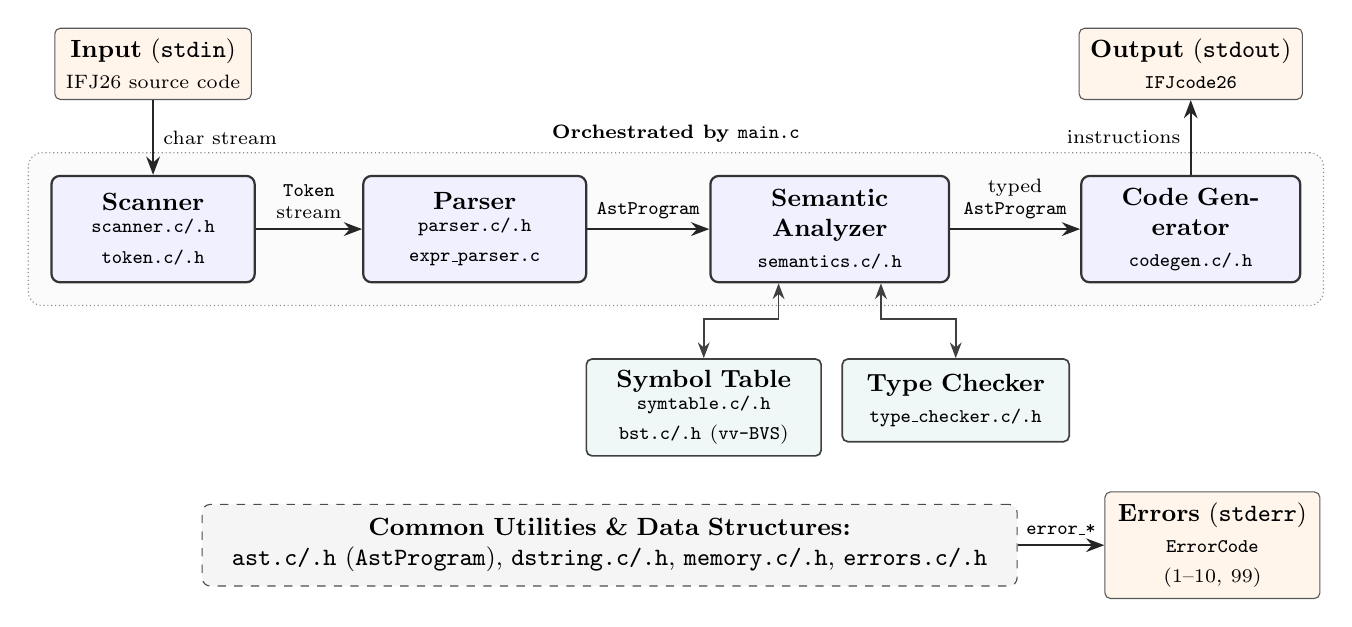
\begin{tikzpicture}[
    font=\small,
    >=Stealth,
    module/.style={
      rectangle, draw=black!80, thick, rounded corners=3pt,
      fill=blue!6, align=center, minimum height=1.35cm, inner sep=4pt
    },
    submod/.style={
      rectangle, draw=black!75, semithick, rounded corners=2pt,
      fill=teal!6, align=center, minimum height=1.05cm, inner sep=4pt
    },
    common/.style={
      rectangle, draw=black!70, dashed, rounded corners=3pt,
      fill=gray!8, align=center, minimum height=0.95cm, inner sep=5pt
    },
    io/.style={
      rectangle, draw=black!65, rounded corners=2pt,
      fill=orange!8, align=center, minimum height=0.85cm, inner sep=4pt
    },
    flow/.style={->, thick, draw=black!85},
    biflow/.style={<->, semithick, draw=black!75},
    lbl/.style={font=\scriptsize, align=center}
  ]
  % Main 4 compiler modules in a horizontal row
  \node[module, text width=2.3cm] (scanner) {
    \textbf{Scanner}\\
    \scriptsize\texttt{scanner.c/.h}\\
    \scriptsize\texttt{token.c/.h}
  };
  \node[module, text width=2.55cm, right=1.35cm of scanner] (parser) {
    \textbf{Parser}\\
    \scriptsize\texttt{parser.c/.h}\\
    \scriptsize\texttt{expr\_parser.c}
  };
  \node[module, text width=2.75cm, right=1.55cm of parser] (sem) {
    \textbf{Semantic Analyzer}\\
    \scriptsize\texttt{semantics.c/.h}
  };
  \node[module, text width=2.5cm, right=1.65cm of sem] (gen) {
    \textbf{Code Generator}\\
    \scriptsize\texttt{codegen.c/.h}
  };
  % Inputs and outputs above the row
  \node[io, above=0.95cm of scanner] (stdin_node) {
    \textbf{Input} (\texttt{stdin})\\
    \scriptsize IFJ26 source code
  };
  \node[io, above=0.95cm of gen] (stdout_node) {
    \textbf{Output} (\texttt{stdout})\\
    \scriptsize\texttt{IFJcode26}
  };
  % Supporting modules below Semantic Analyzer
  \node[submod, text width=2.7cm, below=0.95cm of sem, xshift=-1.6cm] (symtab) {
    \textbf{Symbol Table}\\
    \scriptsize\texttt{symtable.c/.h}\\
    \scriptsize\texttt{bst.c/.h} (\texttt{vv-BVS})
  };
  \node[submod, text width=2.6cm, below=0.95cm of sem, xshift=1.6cm] (typechk) {
    \textbf{Type Checker}\\
    \scriptsize\texttt{type\_checker.c/.h}
  };
  % Driver box enclosing the 4 main modules
  \begin{scope}[on background layer]
    \node[draw=black!45, densely dotted, rounded corners=5pt, fill=gray!3,
          fit=(scanner)(parser)(sem)(gen), inner sep=8pt,
          label={[font=\scriptsize\bfseries, anchor=south]north:Orchestrated by \texttt{main.c}}] (driver) {};
  \end{scope}
  % Common layer at the bottom aligned nicely under the pipeline
  \node[common, text width=10.0cm, below=2.8cm of $(parser.south)!0.38!(sem.south)$] (common) {
    \textbf{Common Utilities \& Data Structures:}\\
    \texttt{ast.c/.h} (\texttt{AstProgram}), \texttt{dstring.c/.h},
    \texttt{memory.c/.h}, \texttt{errors.c/.h}
  };
  \node[io, right=1.1cm of common, text width=2.45cm] (stderr_node) {
    \textbf{Errors} (\texttt{stderr})\\
    \scriptsize\texttt{ErrorCode} (1--10, 99)
  };
  % Data-flow arrows
  \draw[flow] (stdin_node) -- node[lbl, right] {char stream} (scanner);
  \draw[flow] (scanner) -- node[lbl, above] {\texttt{Token}\\stream} (parser);
  \draw[flow] (parser) -- node[lbl, above] {\texttt{AstProgram}} (sem);
  \draw[flow] (sem) -- node[lbl, above] {typed\\\texttt{AstProgram}} (gen);
  \draw[flow] (gen) -- node[lbl, left] {instructions} (stdout_node);
  % Semantic internal interactions
  \draw[biflow] ([xshift=-0.65cm]sem.south) -- ++(0,-0.45) -| (symtab.north);
  \draw[biflow] ([xshift=0.65cm]sem.south) -- ++(0,-0.45) -| (typechk.north);
  % Error output from common layer
  \draw[flow] (common) -- node[lbl, above] {\texttt{error\_*}} (stderr_node);
  \end{tikzpicture}
  \caption{Block diagram of the IFJ26 compiler architecture and data flow between modules.}
  \label{fig:architecture}
\end{figure}

The whole process is orchestrated by \texttt{main.c} which reads \texttt{stdin}.
\texttt{Scanner} then sends a stream of \texttt{Token} structures to \texttt{Parser}.
\texttt{Parser} creates an abstract syntax tree.
\texttt{Semantic analyzer} then does type checking and adds types to AST nodes.
\texttt{Code generator} then takes the typed AST and writes the IFJcode26 on \texttt{stdout}.
If any error occurs, the compiler ends with the corresponding error code from \texttt{errors.h} and frees any used memory.
\subsection{Lexical analysis}

TODO: BALINT

\subsection{Syntactical analysis}

\subsubsection{Main LL(1) parser (\texttt{parser.h}, \texttt{parser.c}, \texttt{parser\_internal.h})}

Function \texttt{parser\_run} implements a recursive descent with one lookahead token from scanner.
It checks the prolog \texttt{import ifj26.*} and processes definitions of functions and extension blocks.
It builds\texttt{AstProgram} or returns syntax error.

\subsubsection{Blocks and commands}

Block structures are controlled by \texttt{INDENT} and texttt{DEDENT}.
For commands starting with an identifier \texttt{parse\_id\_statement} decides by the following \texttt{=} if it is an assignment or an expression.

\subsubsection{Precedence analysis of expressions (\texttt{expr\_parser.c})}

Expressions are processed by stack automaton, that is doing so according to the precedence table, which distinguishes between unary and binary operators.


\subsubsection*{Precedence table}
\begin{table}[htbp]
  \centering
  \small
  \begin{tabular}{@{}l|*{11}{c}@{}}
    \toprule
    & \term{u} & \term{*/} & \term{+-} & \term{rel} & \term{eq} & \term{\&\&} & \term{||} & \term{(} & \term{)} & \term{i} & \term{\$} \\
    \midrule
    \term{u} & $<$ & $>$ & $>$ & $>$ & $>$ & $>$ & $>$ & $<$ & $>$ & $<$ & $>$ \\
    \term{*/} & $<$ & $>$ & $>$ & $>$ & $>$ & $>$ & $>$ & $<$ & $>$ & $<$ & $>$ \\
    \term{+-} & $<$ & $<$ & $>$ & $>$ & $>$ & $>$ & $>$ & $<$ & $>$ & $<$ & $>$ \\
    \term{rel} & $<$ & $<$ & $<$ &  & $>$ & $>$ & $>$ & $<$ & $>$ & $<$ & $>$ \\
    \term{eq} & $<$ & $<$ & $<$ & $<$ &  & $>$ & $>$ & $<$ & $>$ & $<$ & $>$ \\
    \term{\&\&} & $<$ & $<$ & $<$ & $<$ & $<$ & $>$ & $>$ & $<$ & $>$ & $<$ & $>$ \\
    \term{||} & $<$ & $<$ & $<$ & $<$ & $<$ & $<$ & $>$ & $<$ & $>$ & $<$ & $>$ \\
    \term{(} & $<$ & $<$ & $<$ & $<$ & $<$ & $<$ & $<$ & $<$ & $=$ & $<$ &  \\
    \term{)} &  & $>$ & $>$ & $>$ & $>$ & $>$ & $>$ &  & $>$ &  & $>$ \\
    \term{i} &  & $>$ & $>$ & $>$ & $>$ & $>$ & $>$ &  & $>$ &  & $>$ \\
    \term{\$} & $<$ & $<$ & $<$ & $<$ & $<$ & $<$ & $<$ & $<$ &  & $<$ & \textbf{END} \\
    \bottomrule
  \end{tabular}
  \caption{Operator precedence table for expression parsing.}
  \label{tab:precedence}
\end{table}

\newpage
\subsubsection*{LL grammar}
{\footnotesize
\setlength{\tabcolsep}{4pt}
\begin{longtable}{@{}r >{\raggedright\arraybackslash}p{9.2cm} >{\raggedright\arraybackslash}p{6.5cm}@{}}
  \toprule
  \textbf{\#} & \textbf{Production} & \textbf{Predict set} \\
  \midrule
  \endfirsthead
  \toprule
  \textbf{\#} & \textbf{Production} & \textbf{Predict set} \\
  \midrule
  \endhead
  \bottomrule
  \endfoot
  1. & \nt{program} $\to$ \nt{prolog} \nt{definitions} \term{EOF} & --- \\
  2. & \nt{prolog} $\to$ \term{IMPORT} \term{ID} \term{DOT} \term{MUL} \term{EOL} & --- \\
  3. & \nt{definitions} $\to$ \nt{function} \nt{definitions} & \{ \term{DEF}, \term{AT\_MAIN} \} \\
  4. & \nt{definitions} $\to$ $\varepsilon$ & \{ \term{EOF} \} \\
  5. & \nt{function} $\to$ \nt{opt\_main} \term{DEF} \term{ID} \nt{param\_lists} \nt{opt\_type} \term{ASSIGN} \nt{function\_body} & --- \\
  5.1. & \nt{opt\_main} $\to$ \term{AT\_MAIN} \nt{opt\_eol} & \{ \term{AT\_MAIN} \} \\
  5.2. & \nt{opt\_main} $\to$ $\varepsilon$ & \{ \term{DEF} \} \\
  5.3. & \nt{opt\_eol} $\to$ \term{EOL} & \{ \term{EOL} \} \\
  5.4. & \nt{opt\_eol} $\to$ $\varepsilon$ & \{ \term{DEF} \} \\
  6. & \nt{opt\_type} $\to$ \term{COLON} \nt{type} & \{ \term{COLON} \} \\
  7. & \nt{opt\_type} $\to$ $\varepsilon$ & \{ \term{ASSIGN} \} \\
  8. & \nt{type} $\to$ \term{INT} & \{ \term{INT} \} \\
  9. & \nt{type} $\to$ \term{DOUBLE} & \{ \term{DOUBLE} \} \\
  10. & \nt{type} $\to$ \term{STRING} & \{ \term{STRING} \} \\
  11. & \nt{type} $\to$ \term{UNIT} & \{ \term{UNIT} \} \\
  12. & \nt{type} $\to$ \term{BOOLEAN} & \{ \term{BOOLEAN} \} \\
  13. & \nt{parameters} $\to$ \nt{parameter} \nt{parameters\_next} & \{ \term{ID} \} \\
  14. & \nt{parameters} $\to$ $\varepsilon$ & \{ \term{RIGHT\_PAREN} \} \\
  15. & \nt{parameters\_next} $\to$ \term{COMMA} \nt{param\_after\_comma} & \{ \term{COMMA} \} \\
  16. & \nt{parameters\_next} $\to$ $\varepsilon$ & \{ \term{RIGHT\_PAREN} \} \\
  17. & \nt{parameter} $\to$ \term{ID} \term{COLON} \nt{type} & --- \\
  18. & \nt{block} $\to$ \term{INDENT} \nt{statement} \nt{statement\_next} \term{DEDENT} & --- \\
  19. & \nt{statement\_next} $\to$ \nt{statement} \nt{statement\_next} & \{ \term{VAR}, \term{VAL}, \term{WHILE}, \term{IF}, \term{FOR}, \term{RETURN}, \term{ID}, \term{INT\_LIT}, \term{DOUBLE\_LIT}, \term{STRING\_LIT}, \term{TRUE}, \term{FALSE}, \term{LEFT\_PAREN}, \term{ISTRING\_BEGIN} \} \\
  20. & \nt{statement\_next} $\to$ $\varepsilon$ & \{ \term{DEDENT} \} \\
  21. & \nt{statement} $\to$ \nt{var\_def} \nt{stmt\_end} & \{ \term{VAR}, \term{VAL} \} \\
  22. & \nt{var\_def} $\to$ \term{VAR} \term{ID} \nt{opt\_type} \term{ASSIGN} \nt{rhs} & \{ \term{VAR} \} \\
  23. & \nt{var\_def} $\to$ \term{VAL} \term{ID} \nt{opt\_type} \term{ASSIGN} \nt{rhs} & \{ \term{VAL} \} \\
  24. & \nt{statement} $\to$ \nt{while\_stmt} & \{ \term{WHILE} \} \\
  25. & \nt{statement} $\to$ \nt{if\_stmt} & \{ \term{IF} \} \\
  26. & \nt{while\_stmt} $\to$ \term{WHILE} \textit{expr} \term{DO} \term{EOL} \nt{block} & --- \\
  27. & \nt{if\_stmt} $\to$ \term{IF} \textit{expr} \term{THEN} \nt{branch\_body} \nt{opt\_else} & \{ \term{IF} \} \\
  28. & \nt{opt\_else} $\to$ \term{ELSE} \nt{else\_tail} & \{ \term{ELSE} \} \\
  29. & \nt{opt\_else} $\to$ $\varepsilon$ & \{ \term{VAR}, \term{VAL}, \term{WHILE}, \term{IF}, \term{FOR}, \term{RETURN}, \term{ID}, \term{INT\_LIT}, \term{DOUBLE\_LIT}, \term{STRING\_LIT}, \term{TRUE}, \term{FALSE}, \term{LEFT\_PAREN}, \term{ISTRING\_BEGIN}, \term{DEDENT} \} \\
  30. & \nt{else\_tail} $\to$ \nt{branch\_body} & \{ \term{EOL}, \term{RETURN}, \term{ID}, \term{INT\_LIT}, \term{DOUBLE\_LIT}, \term{STRING\_LIT}, \term{TRUE}, \term{FALSE}, \term{LEFT\_PAREN}, \term{MINUS}, \term{NOT}, \term{ISTRING\_BEGIN} \} \\
  31. & \nt{else\_tail} $\to$ \nt{if\_stmt} & \{ \term{IF} \} \\
  32. & \nt{statement} $\to$ \term{RETURN} \nt{opt\_expr} \nt{stmt\_end} & \{ \term{RETURN} \} \\
  33. & \nt{opt\_expr} $\to$ \textit{expr} & \{ \term{ID}, \term{INT\_LIT}, \term{DOUBLE\_LIT}, \term{STRING\_LIT}, \term{TRUE}, \term{FALSE}, \term{LEFT\_PAREN}, \term{MINUS}, \term{NOT}, \term{IF}, \term{ISTRING\_BEGIN} \} \\
  34. & \nt{opt\_expr} $\to$ $\varepsilon$ & \{ \term{EOL}, \term{SEMICOLON}, \term{ELSE} \} \\
  35. & \nt{statement} $\to$ \term{ID} \nt{id\_tail} \nt{stmt\_end} & \{ \term{ID} \} \\
  36. & \nt{id\_tail} $\to$ \term{ASSIGN} \nt{rhs} & \{ \term{ASSIGN} \} \\
  37. & \nt{id\_tail} $\to$ \nt{expr\_rest} & \{ \term{LEFT\_PAREN}, \term{DOT}, \term{PLUS}, \term{MINUS}, \term{MUL}, \term{DIV}, \term{LESS}, \term{LESS\_EQUAL}, \term{GREATER}, \term{GREATER\_EQUAL}, \term{EQUAL}, \term{NOT\_EQUAL}, \term{AND}, \term{OR}, \term{EOL}, \term{SEMICOLON}, \term{ELSE} \} \\
  38. & \nt{statement} $\to$ \textit{expr} \nt{stmt\_end} & \{ \term{INT\_LIT}, \term{DOUBLE\_LIT}, \term{STRING\_LIT}, \term{TRUE}, \term{FALSE}, \term{LEFT\_PAREN}, \term{ISTRING\_BEGIN} \} \\
  39. & \nt{function\_body} $\to$ \term{EOL} \nt{block} & \{ \term{EOL} \} \\
  40. & \nt{function\_body} $\to$ \textit{expr} \term{EOL} & \{ \term{ID}, \term{INT\_LIT}, \term{DOUBLE\_LIT}, \term{STRING\_LIT}, \term{TRUE}, \term{FALSE}, \term{LEFT\_PAREN}, \term{MINUS}, \term{NOT}, \term{IF}, \term{ISTRING\_BEGIN} \} \\
  41. & \nt{stmt\_end} $\to$ \term{EOL} & \{ \term{EOL} \} \\
  42. & \nt{stmt\_end} $\to$ \term{SEMICOLON} & \{ \term{SEMICOLON} \} \\
  43. & \nt{param\_after\_comma} $\to$ \nt{parameter} \nt{parameters\_next} & \{ \term{ID} \} \\
  44. & \nt{param\_after\_comma} $\to$ $\varepsilon$ & \{ \term{RIGHT\_PAREN} \} \\
  45. & \nt{param\_lists} $\to$ \term{LEFT\_PAREN} \nt{parameters} \term{RIGHT\_PAREN} \nt{param\_lists} & \{ \term{LEFT\_PAREN} \} \\
  46. & \nt{param\_lists} $\to$ $\varepsilon$ & \{ \term{COLON}, \term{ASSIGN} \} \\
  47. & \nt{definitions} $\to$ \nt{extension} \nt{definitions} & \{ \term{EXTENSION} \} \\
  48. & \nt{extension} $\to$ \term{EXTENSION} \term{LEFT\_PAREN} \nt{parameter} \term{RIGHT\_PAREN} \term{EOL} \term{INDENT} \nt{method} \nt{methods\_next} \term{DEDENT} & --- \\
  49. & \nt{method} $\to$ \term{DEF} \term{ID} \nt{param\_lists} \nt{opt\_type} \term{ASSIGN} \nt{function\_body} & --- \\
  50. & \nt{methods\_next} $\to$ \nt{method} \nt{methods\_next} & \{ \term{DEF} \} \\
  51. & \nt{methods\_next} $\to$ $\varepsilon$ & \{ \term{DEDENT} \} \\
  52. & \nt{type} $\to$ \term{LEFT\_PAREN} \nt{type\_list} \term{RIGHT\_PAREN} \term{BIG\_ARR} \nt{type} & \{ \term{LEFT\_PAREN} \} \\
  53. & \nt{type\_list} $\to$ \nt{type} \nt{type\_next} & \{ \term{INT}, \term{DOUBLE}, \term{STRING}, \term{UNIT}, \term{BOOLEAN}, \term{LEFT\_PAREN} \} \\
  54. & \nt{type\_list} $\to$ $\varepsilon$ & \{ \term{RIGHT\_PAREN} \} \\
  55. & \nt{type\_next} $\to$ \term{COMMA} \nt{type} \nt{type\_next} & \{ \term{COMMA} \} \\
  56. & \nt{type\_next} $\to$ $\varepsilon$ & \{ \term{RIGHT\_PAREN} \} \\
  57. & \nt{branch\_body} $\to$ \term{EOL} \nt{block} & \{ \term{EOL} \} \\
  58. & \nt{branch\_body} $\to$ \term{RETURN} \nt{opt\_expr} & \{ \term{RETURN} \} \\
  59. & \nt{branch\_body} $\to$ \term{ID} \nt{id\_tail} & \{ \term{ID} \} \\
  60. & \nt{branch\_body} $\to$ \textit{expr} & \{ \term{INT\_LIT}, \term{DOUBLE\_LIT}, \term{STRING\_LIT}, \term{TRUE}, \term{FALSE}, \term{LEFT\_PAREN}, \term{MINUS}, \term{NOT}, \term{ISTRING\_BEGIN} \} \\
  61. & \nt{statement} $\to$ \nt{for\_stmt} \nt{stmt\_end} & \{ \term{FOR} \} \\
  62. & \nt{for\_stmt} $\to$ \term{FOR} \nt{for\_header} \term{DO} \nt{branch\_body} & --- \\
  63. & \nt{for\_header} $\to$ \nt{generator} \nt{guards} & \{ \term{ID} \} \\
  64. & \nt{for\_header} $\to$ \term{EOL} \term{INDENT} \nt{generator} \term{EOL} \nt{guard\_lines} \term{DEDENT} & \{ \term{EOL} \} \\
  65. & \nt{generator} $\to$ \term{ID} \term{LEFT\_ARR} \textit{expr} \nt{range} & --- \\
  66. & \nt{range} $\to$ \term{TO} \textit{expr} \nt{opt\_by} & \{ \term{TO} \} \\
  67. & \nt{range} $\to$ \term{UNTIL} \textit{expr} & \{ \term{UNTIL} \} \\
  68. & \nt{opt\_by} $\to$ \term{BY} \textit{expr} & \{ \term{BY} \} \\
  69. & \nt{opt\_by} $\to$ $\varepsilon$ & \{ \term{IF}, \term{DO}, \term{EOL} \} \\
  70. & \nt{guards} $\to$ \term{IF} \textit{expr} \nt{guards} & \{ \term{IF} \} \\
  71. & \nt{guards} $\to$ $\varepsilon$ & \{ \term{DO} \} \\
  72. & \nt{guard\_lines} $\to$ \term{IF} \textit{expr} \term{EOL} \nt{guard\_lines} & \{ \term{IF} \} \\
  73. & \nt{guard\_lines} $\to$ $\varepsilon$ & \{ \term{DEDENT} \} \\
  74. & \nt{rhs} $\to$ \textit{expr} & \{ \term{ID}, \term{INT\_LIT}, \term{DOUBLE\_LIT}, \term{STRING\_LIT}, \term{TRUE}, \term{FALSE}, \term{LEFT\_PAREN}, \term{MINUS}, \term{NOT}, \term{IF}, \term{ISTRING\_BEGIN} \} \\
  75. & \nt{rhs} $\to$ \term{EOL} \term{INDENT} \textit{expr} \nt{stmt\_end} \term{DEDENT} & \{ \term{EOL} \} \\
  76. & \nt{stmt\_end} $\to$ $\varepsilon$ & \{ \term{VAR}, \term{VAL}, \term{WHILE}, \term{IF}, \term{FOR}, \term{RETURN}, \term{ID}, \term{INT\_LIT}, \term{DOUBLE\_LIT}, \term{STRING\_LIT}, \term{TRUE}, \term{FALSE}, \term{LEFT\_PAREN}, \term{ISTRING\_BEGIN}, \term{DEDENT} \} \\
  77. & \nt{lambda} $\to$ \term{LEFT\_PAREN} \nt{parameters} \term{RIGHT\_PAREN} \term{BIG\_ARR} \nt{lambda\_body} & --- \\
  78. & \nt{lambda\_body} $\to$ \term{EOL} \nt{block} & \{ \term{EOL} \} \\
  79. & \nt{lambda\_body} $\to$ \textit{expr} & \{ \term{ID}, \term{INT\_LIT}, \term{DOUBLE\_LIT}, \term{STRING\_LIT}, \term{TRUE}, \term{FALSE}, \term{LEFT\_PAREN}, \term{MINUS}, \term{NOT}, \term{IF}, \term{ISTRING\_BEGIN} \} \\
  80. & \nt{if\_expr} $\to$ \term{IF} \textit{expr} \term{THEN} \nt{branch\_body} \term{ELSE} \nt{else\_tail} & --- \\
  81. & \nt{istring} $\to$ \term{ISTRING\_BEGIN} \nt{istring\_parts} \term{ISTRING\_END} & --- \\
  82. & \nt{istring\_parts} $\to$ \term{ISTRING\_PART} \nt{istring\_parts} & \{ \term{ISTRING\_PART} \} \\
  83. & \nt{istring\_parts} $\to$ \term{ISTRING\_ID} \nt{istring\_parts} & \{ \term{ISTRING\_ID} \} \\
  84. & \nt{istring\_parts} $\to$ \term{ISTRING\_EXPR\_BEGIN} \textit{expr} \term{ISTRING\_EXPR\_END} \nt{istring\_parts} & \{ \term{ISTRING\_EXPR\_BEGIN} \} \\
  85. & \nt{istring\_parts} $\to$ $\varepsilon$ & \{ \term{ISTRING\_END} \} \\
  86. & \nt{postfix} $\to$ \term{LEFT\_PAREN} \nt{arguments} \term{RIGHT\_PAREN} \nt{postfix} & \{ \term{LEFT\_PAREN} \} \\
  87. & \nt{postfix} $\to$ \term{DOT} \term{ID} \nt{postfix} & \{ \term{DOT} \} \\
  88. & \nt{postfix} $\to$ $\varepsilon$ & \{ \term{PLUS}, \term{MINUS}, \term{MUL}, \term{DIV}, \term{LESS}, \term{LESS\_EQUAL}, \term{GREATER}, \term{GREATER\_EQUAL}, \term{EQUAL}, \term{NOT\_EQUAL}, \term{AND}, \term{OR}, \term{RIGHT\_PAREN}, \term{COMMA}, \term{EOL}, \term{SEMICOLON}, \term{EOF}, \term{THEN}, \term{DO}, \term{ELSE}, \term{TO}, \term{UNTIL}, \term{BY}, \term{IF}, \term{ISTRING\_EXPR\_END} \} \\
  89. & \nt{arguments} $\to$ \textit{expr} \nt{arguments\_next} & \{ \term{ID}, \term{INT\_LIT}, \term{DOUBLE\_LIT}, \term{STRING\_LIT}, \term{TRUE}, \term{FALSE}, \term{LEFT\_PAREN}, \term{MINUS}, \term{NOT}, \term{IF}, \term{ISTRING\_BEGIN} \} \\
  90. & \nt{arguments} $\to$ $\varepsilon$ & \{ \term{RIGHT\_PAREN} \} \\
  91. & \nt{arguments\_next} $\to$ \term{COMMA} \nt{arg\_after\_comma} & \{ \term{COMMA} \} \\
  92. & \nt{arguments\_next} $\to$ $\varepsilon$ & \{ \term{RIGHT\_PAREN} \} \\
  93. & \nt{arg\_after\_comma} $\to$ \textit{expr} \nt{arguments\_next} & \{ \term{ID}, \term{INT\_LIT}, \term{DOUBLE\_LIT}, \term{STRING\_LIT}, \term{TRUE}, \term{FALSE}, \term{LEFT\_PAREN}, \term{MINUS}, \term{NOT}, \term{IF}, \term{ISTRING\_BEGIN} \} \\
  94. & \nt{arg\_after\_comma} $\to$ $\varepsilon$ & \{ \term{RIGHT\_PAREN} \} \\
\end{longtable}
}

\subsubsection*{LL table}
{\footnotesize
\setlength{\tabcolsep}{4pt}
\begin{longtable}{@{}l >{\raggedright\arraybackslash}p{12.6cm}@{}}
  \toprule
  \textbf{Nonterminal} & \textbf{Lookahead token $\to$ rule number} \\
  \midrule
  \endfirsthead
  \toprule
  \textbf{Nonterminal} & \textbf{Lookahead token $\to$ rule number} \\
  \midrule
  \endhead
  \bottomrule
  \endfoot
  \nt{program} & \term{IMPORT}~$\to$~1 \\
  \nt{prolog} & \term{IMPORT}~$\to$~2 \\
  \nt{definitions} & \term{DEF}~$\to$~3, \term{AT\_MAIN}~$\to$~3, \term{EXTENSION}~$\to$~47, \term{EOF}~$\to$~4 \\
  \nt{function} & \term{AT\_MAIN}~$\to$~5, \term{DEF}~$\to$~5 \\
  \nt{opt\_main} & \term{AT\_MAIN}~$\to$~5.1, \term{DEF}~$\to$~5.2 \\
  \nt{opt\_eol} & \term{EOL}~$\to$~5.3, \term{DEF}~$\to$~5.4 \\
  \nt{opt\_type} & \term{COLON}~$\to$~6, \term{ASSIGN}~$\to$~7 \\
  \nt{type} & \term{INT}~$\to$~8, \term{DOUBLE}~$\to$~9, \term{STRING}~$\to$~10, \term{UNIT}~$\to$~11, \term{BOOLEAN}~$\to$~12, \term{LEFT\_PAREN}~$\to$~52 \\
  \nt{parameters} & \term{ID}~$\to$~13, \term{RIGHT\_PAREN}~$\to$~14 \\
  \nt{parameters\_next} & \term{COMMA}~$\to$~15, \term{RIGHT\_PAREN}~$\to$~16 \\
  \nt{param\_after\_comma} & \term{ID}~$\to$~43, \term{RIGHT\_PAREN}~$\to$~44 \\
  \nt{parameter} & \term{ID}~$\to$~17 \\
  \nt{param\_lists} & \term{LEFT\_PAREN}~$\to$~45, \term{COLON}~$\to$~46, \term{ASSIGN}~$\to$~46 \\
  \nt{extension} & \term{EXTENSION}~$\to$~48 \\
  \nt{method} & \term{DEF}~$\to$~49 \\
  \nt{methods\_next} & \term{DEF}~$\to$~50, \term{DEDENT}~$\to$~51 \\
  \nt{type\_list} & \term{INT}~$\to$~53, \term{DOUBLE}~$\to$~53, \term{STRING}~$\to$~53, \term{UNIT}~$\to$~53, \term{BOOLEAN}~$\to$~53, \term{LEFT\_PAREN}~$\to$~53, \term{RIGHT\_PAREN}~$\to$~54 \\
  \nt{type\_next} & \term{COMMA}~$\to$~55, \term{RIGHT\_PAREN}~$\to$~56 \\
  \nt{function\_body} & \term{EOL}~$\to$~39, \term{ID}~$\to$~40, \term{INT\_LIT}~$\to$~40, \term{DOUBLE\_LIT}~$\to$~40, \term{STRING\_LIT}~$\to$~40, \term{TRUE}~$\to$~40, \term{FALSE}~$\to$~40, \term{LEFT\_PAREN}~$\to$~40, \term{MINUS}~$\to$~40, \term{NOT}~$\to$~40, \term{IF}~$\to$~40, \term{ISTRING\_BEGIN}~$\to$~40 \\
  \nt{block} & \term{INDENT}~$\to$~18 \\
  \nt{statement\_next} & \term{VAR}~$\to$~19, \term{VAL}~$\to$~19, \term{WHILE}~$\to$~19, \term{IF}~$\to$~19, \term{FOR}~$\to$~19, \term{RETURN}~$\to$~19, \term{ID}~$\to$~19, \term{INT\_LIT}~$\to$~19, \term{DOUBLE\_LIT}~$\to$~19, \term{STRING\_LIT}~$\to$~19, \term{TRUE}~$\to$~19, \term{FALSE}~$\to$~19, \term{LEFT\_PAREN}~$\to$~19, \term{ISTRING\_BEGIN}~$\to$~19, \term{DEDENT}~$\to$~20 \\
  \nt{statement} & \term{VAR}~$\to$~21, \term{VAL}~$\to$~21, \term{WHILE}~$\to$~24, \term{IF}~$\to$~25, \term{RETURN}~$\to$~32, \term{ID}~$\to$~35, \term{INT\_LIT}~$\to$~38, \term{DOUBLE\_LIT}~$\to$~38, \term{STRING\_LIT}~$\to$~38, \term{TRUE}~$\to$~38, \term{FALSE}~$\to$~38, \term{LEFT\_PAREN}~$\to$~38, \term{ISTRING\_BEGIN}~$\to$~38, \term{FOR}~$\to$~61 \\
  \nt{stmt\_end} & \term{EOL}~$\to$~41, \term{SEMICOLON}~$\to$~42, \term{VAR}~$\to$~76, \term{VAL}~$\to$~76, \term{WHILE}~$\to$~76, \term{IF}~$\to$~76, \term{FOR}~$\to$~76, \term{RETURN}~$\to$~76, \term{ID}~$\to$~76, \term{INT\_LIT}~$\to$~76, \term{DOUBLE\_LIT}~$\to$~76, \term{STRING\_LIT}~$\to$~76, \term{TRUE}~$\to$~76, \term{FALSE}~$\to$~76, \term{LEFT\_PAREN}~$\to$~76, \term{ISTRING\_BEGIN}~$\to$~76, \term{DEDENT}~$\to$~76 \\
  \nt{var\_def} & \term{VAR}~$\to$~22, \term{VAL}~$\to$~23 \\
  \nt{rhs} & \term{ID}~$\to$~74, \term{INT\_LIT}~$\to$~74, \term{DOUBLE\_LIT}~$\to$~74, \term{STRING\_LIT}~$\to$~74, \term{TRUE}~$\to$~74, \term{FALSE}~$\to$~74, \term{LEFT\_PAREN}~$\to$~74, \term{MINUS}~$\to$~74, \term{NOT}~$\to$~74, \term{IF}~$\to$~74, \term{ISTRING\_BEGIN}~$\to$~74, \term{EOL}~$\to$~75 \\
  \nt{while\_stmt} & \term{WHILE}~$\to$~26 \\
  \nt{if\_stmt} & \term{IF}~$\to$~27 \\
  \nt{opt\_else} & \term{ELSE}~$\to$~28, \term{VAR}~$\to$~29, \term{VAL}~$\to$~29, \term{WHILE}~$\to$~29, \term{IF}~$\to$~29, \term{FOR}~$\to$~29, \term{RETURN}~$\to$~29, \term{ID}~$\to$~29, \term{INT\_LIT}~$\to$~29, \term{DOUBLE\_LIT}~$\to$~29, \term{STRING\_LIT}~$\to$~29, \term{TRUE}~$\to$~29, \term{FALSE}~$\to$~29, \term{LEFT\_PAREN}~$\to$~29, \term{ISTRING\_BEGIN}~$\to$~29, \term{DEDENT}~$\to$~29 \\
  \nt{else\_tail} & \term{EOL}~$\to$~30, \term{RETURN}~$\to$~30, \term{ID}~$\to$~30, \term{INT\_LIT}~$\to$~30, \term{DOUBLE\_LIT}~$\to$~30, \term{STRING\_LIT}~$\to$~30, \term{TRUE}~$\to$~30, \term{FALSE}~$\to$~30, \term{LEFT\_PAREN}~$\to$~30, \term{MINUS}~$\to$~30, \term{NOT}~$\to$~30, \term{ISTRING\_BEGIN}~$\to$~30, \term{IF}~$\to$~31 \\
  \nt{branch\_body} & \term{EOL}~$\to$~57, \term{RETURN}~$\to$~58, \term{ID}~$\to$~59, \term{INT\_LIT}~$\to$~60, \term{DOUBLE\_LIT}~$\to$~60, \term{STRING\_LIT}~$\to$~60, \term{TRUE}~$\to$~60, \term{FALSE}~$\to$~60, \term{LEFT\_PAREN}~$\to$~60, \term{MINUS}~$\to$~60, \term{NOT}~$\to$~60, \term{ISTRING\_BEGIN}~$\to$~60 \\
  \nt{for\_stmt} & \term{FOR}~$\to$~62 \\
  \nt{for\_header} & \term{ID}~$\to$~63, \term{EOL}~$\to$~64 \\
  \nt{generator} & \term{ID}~$\to$~65 \\
  \nt{range} & \term{TO}~$\to$~66, \term{UNTIL}~$\to$~67 \\
  \nt{opt\_by} & \term{BY}~$\to$~68, \term{IF}~$\to$~69, \term{DO}~$\to$~69, \term{EOL}~$\to$~69 \\
  \nt{guards} & \term{IF}~$\to$~70, \term{DO}~$\to$~71 \\
  \nt{guard\_lines} & \term{IF}~$\to$~72, \term{DEDENT}~$\to$~73 \\
  \nt{opt\_expr} & \term{ID}~$\to$~33, \term{INT\_LIT}~$\to$~33, \term{DOUBLE\_LIT}~$\to$~33, \term{STRING\_LIT}~$\to$~33, \term{TRUE}~$\to$~33, \term{FALSE}~$\to$~33, \term{LEFT\_PAREN}~$\to$~33, \term{MINUS}~$\to$~33, \term{NOT}~$\to$~33, \term{IF}~$\to$~33, \term{ISTRING\_BEGIN}~$\to$~33, \term{EOL}~$\to$~34, \term{SEMICOLON}~$\to$~34, \term{ELSE}~$\to$~34 \\
  \nt{id\_tail} & \term{ASSIGN}~$\to$~36, \term{LEFT\_PAREN}~$\to$~37, \term{DOT}~$\to$~37, \term{PLUS}~$\to$~37, \term{MINUS}~$\to$~37, \term{MUL}~$\to$~37, \term{DIV}~$\to$~37, \term{LESS}~$\to$~37, \term{LESS\_EQUAL}~$\to$~37, \term{GREATER}~$\to$~37, \term{GREATER\_EQUAL}~$\to$~37, \term{EQUAL}~$\to$~37, \term{NOT\_EQUAL}~$\to$~37, \term{AND}~$\to$~37, \term{OR}~$\to$~37, \term{EOL}~$\to$~37, \term{SEMICOLON}~$\to$~37, \term{ELSE}~$\to$~37 \\
  \midrule
  \multicolumn{2}{@{}l}{\textbf{Expression operands and postfix rules}} \\
  \midrule
  \nt{lambda} & \term{LEFT\_PAREN}~$\to$~77 \\
  \nt{lambda\_body} & \term{EOL}~$\to$~78, \term{ID}~$\to$~79, \term{INT\_LIT}~$\to$~79, \term{DOUBLE\_LIT}~$\to$~79, \term{STRING\_LIT}~$\to$~79, \term{TRUE}~$\to$~79, \term{FALSE}~$\to$~79, \term{LEFT\_PAREN}~$\to$~79, \term{MINUS}~$\to$~79, \term{NOT}~$\to$~79, \term{IF}~$\to$~79, \term{ISTRING\_BEGIN}~$\to$~79 \\
  \nt{if\_expr} & \term{IF}~$\to$~80 \\
  \nt{istring} & \term{ISTRING\_BEGIN}~$\to$~81 \\
  \nt{istring\_parts} & \term{ISTRING\_PART}~$\to$~82, \term{ISTRING\_ID}~$\to$~83, \term{ISTRING\_EXPR\_BEGIN}~$\to$~84, \term{ISTRING\_END}~$\to$~85 \\
  \nt{postfix} & \term{LEFT\_PAREN}~$\to$~86, \term{DOT}~$\to$~87, \term{PLUS}~$\to$~88, \term{MINUS}~$\to$~88, \term{MUL}~$\to$~88, \term{DIV}~$\to$~88, \term{LESS}~$\to$~88, \term{LESS\_EQUAL}~$\to$~88, \term{GREATER}~$\to$~88, \term{GREATER\_EQUAL}~$\to$~88, \term{EQUAL}~$\to$~88, \term{NOT\_EQUAL}~$\to$~88, \term{AND}~$\to$~88, \term{OR}~$\to$~88, \term{RIGHT\_PAREN}~$\to$~88, \term{COMMA}~$\to$~88, \term{EOL}~$\to$~88, \term{SEMICOLON}~$\to$~88, \term{EOF}~$\to$~88, \term{THEN}~$\to$~88, \term{DO}~$\to$~88, \term{ELSE}~$\to$~88, \term{TO}~$\to$~88, \term{UNTIL}~$\to$~88, \term{BY}~$\to$~88, \term{IF}~$\to$~88, \term{ISTRING\_EXPR\_END}~$\to$~88 \\
  \nt{arguments} & \term{ID}~$\to$~89, \term{INT\_LIT}~$\to$~89, \term{DOUBLE\_LIT}~$\to$~89, \term{STRING\_LIT}~$\to$~89, \term{TRUE}~$\to$~89, \term{FALSE}~$\to$~89, \term{LEFT\_PAREN}~$\to$~89, \term{MINUS}~$\to$~89, \term{NOT}~$\to$~89, \term{IF}~$\to$~89, \term{ISTRING\_BEGIN}~$\to$~89, \term{RIGHT\_PAREN}~$\to$~90 \\
  \nt{arguments\_next} & \term{COMMA}~$\to$~91, \term{RIGHT\_PAREN}~$\to$~92 \\
  \nt{arg\_after\_comma} & \term{ID}~$\to$~93, \term{INT\_LIT}~$\to$~93, \term{DOUBLE\_LIT}~$\to$~93, \term{STRING\_LIT}~$\to$~93, \term{TRUE}~$\to$~93, \term{FALSE}~$\to$~93, \term{LEFT\_PAREN}~$\to$~93, \term{MINUS}~$\to$~93, \term{NOT}~$\to$~93, \term{IF}~$\to$~93, \term{ISTRING\_BEGIN}~$\to$~93, \term{RIGHT\_PAREN}~$\to$~94 \\
\end{longtable}
}

\subsection{Semantical analysis}

\subsubsection{Symtable vv-BVS (\texttt{bst.h}, \texttt{bst.c})}

Symtable is implemented as AVL tree in \texttt{bst.c} and \texttt{bst.h}.
When inserting a new node, height is checked and made sure, that tree isn't degraded to a list. There are 4 rotation operations, they ensure time complexity stays $O(\log n)$.
\texttt{SymbolData} define whether a function or variable was saved.

Scopes are part of single-linked stack via a \texttt{parent} pointer.
When entering a block a \texttt{symtable\_push\_scope} is called.
When exiting a block a \texttt{symtable\_pop\_scope} is called.

\subsubsection{Two pass semantic analysis (\texttt{semantics.h}, \texttt{semantics.c})}

It was decided that a two pass semantic analysis will be implemented, because of clear distinction between roles of the first and second pass.
In first pass we only initiate a new symtable with global scope, we insert the IFJ26 built-in functions then any user functions.
In first pass we also check for function redefinitions, correct \texttt{@main} and for duplicate names of functions.
In second pass we go into the bodies of functions, for each we create a new scope.
Then we proceed with the proper semantic analysis.

\subsubsection{System for type checking (\texttt{type\_checker.h}, \texttt{type\_checker.c})}

We have basic atomic types such as \texttt{Int}, \texttt{Double}, \texttt{String} and others and function types \texttt{AST\_TYPE\_FUNCTION}.
Then a type checking control begins, only automatic conversion we need to be aware of is \texttt{Int} $\to$ \texttt{Double}.
\texttt{check\_expression} recursively evaluates types of expression and writes the result into \texttt{expr->evaluated\_type} for code generator.

\subsection{Code generator (\texttt{codegen.h}, \texttt{codegen.c})}

Code generator takes the semantically checked and typed AST and writes the final IFJcode26 into the output stream or returns error 99.
Expression evaluations is built on a data stack.
A unified function calling convention for functions including lambdas passes arguments from left to right through the stack and a local frame is created (\texttt{CREATEFRAME}/\texttt{PUSHFRAME}).
Shadowing is solved by renaming \texttt{LF@<name>\$<uid>}.
Only built-in functions actually used in the program are generated.


\section{Usage of AI}

In our team we agreed that we should be able to use AI if it is allowed and we understand the code it created.
We used AI to generate small, exactly specified parts of code.
We mostly used AI for consulting, explaining difficult concepts, help with Git and GitHub, finding bugs and asking questions.
Specifically we used Google Gemini and Anthropic Claude.
We didn't use AI generated code for forbidden parts of the project.
AI was also partially used to finish Peter's part, so the entire project could at least work.

\subsection{Typical usage of AI}

Typically before any coding, we used AI to explain the topic and concepts we were currently working on.
Then we either wrote pseudocode and asked the AI to remake it or we asked the AI to generate specified small parts of code.
If any errors occurred we used AI for debugging, typically when working with memory.

\subsection{Problems with AI}

When Adam was using AI in different chats, it struggled to understand context. Therefore he had to use a common \texttt{GEMINI.md} where all context was stored along with instructions how AI should behave.

\addcontentsline{toc}{section}{References}
\begin{thebibliography}{9}
  \bibitem{ifj_zadani}
  Ondryáš, O., \& Křivka, Z. (2026).
  \textit{Zadání projektu z předmětů IFJ a IAL} (revize z 8. 10. 2026).
  Brno University of Technology, Faculty of Information Technology.
  \bibitem{ifj_spec}
  Ondryáš, O., \& Křivka, Z. (2026).
  \textit{Specifikace jazyků IFJ26 a IFJcode26 (IFJ/IAL 2026/2027)} (revize z 11. 10. 2026).
  Brno University of Technology, Faculty of Information Technology.
  \bibitem{ifj_lectures}
  Meduna, A., \& Lukáš, R.
  \textit{Formal Languages and Compilers (IFJ)} [Lecture slides].
  Brno University of Technology, Faculty of Information Technology.
  \bibitem{ial_lectures}
  \textit{Algorithms (IAL)} [Course study materials].
  Brno University of Technology, Faculty of Information Technology, 2026.
  \bibitem{scala3}
  École Polytechnique Fédérale de Lausanne (EPFL).
  \textit{Scala 3 Documentation}.
  Available at: \url{https://docs.scala-lang.org/scala3/}
\end{thebibliography}

\end{document}
